\documentclass[12pt,a4paper,oneside,fleqn]{article}

%\usepackage[utf8]{inputenc}
\usepackage{fancyhdr}
\usepackage[inner=20mm,
            outer=20mm,
            top=30mm,
            bottom=30mm]{geometry}
\usepackage{amsfonts,amssymb,amsmath}
\usepackage[shortlabels]{enumitem}
\usepackage[section]{placeins}
\usepackage{float}
\usepackage[slovene]{babel}
\usepackage[cp1250]{inputenc}
\usepackage{graphicx}
\usepackage{abstract}
\usepackage[justification=raggedright,tableposition=top, labelfont=it,font=it]{caption}
\usepackage[numbib]{tocbibind}
\usepackage{mathtools}

\pagenumbering{gobble}

\captionsetup[table]{singlelinecheck=off}


\makeatletter
\def\@maketitle{%
  \newpage
  \null
  \vskip 2em%
  \begin{center}%
  \let \footnote \thanks
    {\fontsize{16pt}{12pt}\selectfont\textbf \@title \par}%
    \vskip 1.5em%
    {\large
      \lineskip .5em%
      \begin{tabular}[t]{c}%
        \fontsize{12pt}{12pt}\emph{\@author}
      \end{tabular}\par}%
    \vskip 1em%
    %{\large \@date}%
  \end{center}%
  \par
  \vskip 1.5em}
\makeatother

% set equation environment indentation
\setlength\parindent{0pt}
\setlength{\mathindent}{0.5cm}



\title{NAVODILA ZA PISANJE PRISPEVKA ZA SRE�ANJE ��TUDENTSKA  TEHNI�KA KONFERENCA - �TeKam�}
\author{doc. dr. Toma� Berlec, doc. dr. Miha Brojan, dr. Bo�tjan Drobni�}


\renewcommand{\absnamepos}{flushleft}

\renewcommand{\abstractnamefont}{\fontsize{16pt}{12pt}\selectfont\textbf}
\setlength{\absleftindent}{0mm}
\setlength{\absrightindent}{0mm}
\renewcommand{\abstracttextfont}{\it}

\setlist[enumerate]{nosep}
\renewcommand{\baselinestretch}{1.2}
\fancypagestyle{plain}{
\fancyhead[LO,LE]{\hspace{1cm}�tudentska tehni�ka konferenca}
\fancyhead[RO,RE]{�TeKam 2019 \hspace{1cm}}
%\renewcommand{\footrulewidth}{0.4pt}
\fancyfootoffset{-6.5cm}
\fancyfoot[CO, CE]{\thepage}

}

\begin{document}
\pagestyle{plain}
\maketitle

\begin{abstract}
V nalogi je obravnavan postopek 3D rekonstukcije objektov na podlagi ve? zajetih slik. Za rekonstrukcijo je uporabljena FBP (angl. \textit{Filtered Backprojection }) metoda. Temelji na rekonstrukciji 3D oblike iz slik, ki so zajete pri znanih kotih zasuka objekta. Velik poudarek je namenjen izgradnji in zasnovi sistema, saj je od njegove postavitve odvisna kakovost zajetih slik.  Osredoto?amo se predvsem na elemente, ki nam pomagajo pri ?imbolj?i rekonstrukciji objekta v obliki oblaka to?k. Prikazana je kalibracija sistema in preslikava slik v metri?ni koordinatni sistem. Predstavljena je uporabnost rekontrukcije objektov in izvedba vzvratnega in?enirstva skeniranega objekta.(ODSTRANI KRATICE)
\end{abstract}


\section{Uvod}
V robotskem vidu in ra?unalni?ki grafiki je 3D rekonstrukcija proces zajemanja oblike in videza realnega objekta. Proces je lahko dose?en z aktivnimi ali pasivnimi metodami. V nalogi je uporabljena pasivna FBP metoda. Uporaba rekonstrukcije lahko dolo?i profil 3D objekta oziroma koordinate katerikoli to?ke na tem profilu. Digitalna slika je v na?em primeru vir informacij. Za dobro rekonstrukcijo je potrebno upo?tevati vizualno dispariteto, osvetlitev, performance kamere in zna?ilnosti scene. Uporabljeno kamero je potrebno ustrezno skalibrirati in merjene to?ke pretvoriti v metri?ni koordinatni sistem. Bolje kot je zastavljen zajem slik, ustreznej?i so kon?ni rezultati. Dobro zajete slike olaj?ajo obdelavo. Rekonstrukcija objektov je uporabljena v razli?nih podro?jih raziskovanja. Med drugim v medicini, robotiki, ra?unalni?kih igrah in v vzvratnem in?enirstvu \cite{vir1,vir2, vir3}. 


%\section{Metode dela in potek raziskave}
\section{Teoreti?no ozadje}

\subsection{Kalibracija}
Pomagamo si z \cite{spic2}. Pred za?etkom izvedbe rekonstrukcije je potrebna geometrijska kalibracija sistema. Namen kalibracije je pridobitev parametrov toge preslikave, ki jih bomo potrebovali kasneje v algoritmu 3D rekonstrukcije s filtrirano povratno projekcijo. Cilj je projekcija iz slikovnega v metri?ni koordinatni sistem. Referen?ne to?ke kalibracijskega objekta (3D) najprej togo premaknemo na mesto rotirajo?e mize. Nato sledi DLT (angl. \textit{Direct Linear Transformation}) kalibracija med 3D to?kami referen?nega kalibra $T_{ref},_i = (X_i, Y_i, Z_i)$ ter 2D naborom to?k kalibra iz slikovnega koordinatnega sistema $t_{slik},_i = (x_i, y_i)$. Pri tem je ?tevilo to?k kalibracijskega objekta $i = 8$. Pri DLT kalibraciji z razcepom na singularne vrednosti re?ujemo slede?i sistem:


\begin{equation}
\setcounter{MaxMatrixCols}{12}
a = 
\begin{bsmallmatrix}
X_1 & Y_1 & Z_1 & 0 & 0 & 0 & -x_1 X_1 & -x_1 Y_1 & -x_1 Z_1 & 1 & 0 & -x_1 \\ 
0 & 0 & 0 & X_1 & Y_1 & Z_1 & -y_1 X_1 & -y_1 Y_1 & -y_1 Z_1 & 0 & 1 & -y_1 \\
 &  &  &  &  &  & \vdots &  &  &  &  &  \\
X_8 & Y_8 & Z_8 & 0 & 0 & 0 & -x_8 X_8 & -x_8 Y_8 & -x_8 Z_8 & 1 & 0 & -x_8 \\ 
0 & 0 & 0 & X_8 & Y_8 & Z_8 & -y_8 X_8 & -y_8 Y_8 & -y_8 Z_8 & 0 & 1 & -y_8 \\
\end{bsmallmatrix}
\end{equation}

%\begin{equation}
%\setcounter{MaxMatrixCols}{12}
%a = 
%\begin{bsmallmatrix}
%X_i & Y_i & Z_i & 0 & 0 & 0 & -x_i X_i & -x_i Y_i & -x_i Z_i & 1 & 0 & -x_i \\ 
%0 & 0 & 0 & X_i & Y_ i& Z_i & -y_i X_i & -y_i Y_i & -y_i Z_i & 0 & 1 & -y_i \\
%\end{bsmallmatrix}
%\end{equation}

\begin{equation}
\setcounter{MaxMatrixCols}{12}
\textbf{p} =
\begin{bsmallmatrix}
r_{11} & r_{12} & r_{13} & r_{21} & r_{22} & r_{23} & r_{31} & r_{23} & r_{33} & t_x & t_y & t_z
\end{bsmallmatrix}
\end{equation}

\begin{equation}
a\textbf{p}^T=0
\end{equation}

Matrika $a$ ima dimenzije $16 \times 12$. Re?itev sistema predstavlja 12 parametrov toge preslikave, ki predstavljajo rotacijo $r_{ij}$ ter translacijo $t_k$.

\subsection{Filtrirana povratna projekcija}

Pomagamo si z \cite{spic1}. Jedro naloge predstavlja postopek FBP (angl. \textit{Filtered Backprojection}), ki je eden od temelnjih na?inov rekonstrukcije pri slikanju z ra?unalni?ko tomografijo na podro?ju zdravstva. Idejo koncepta filtrirane povratne projekcije je najenostavneje predstaviti na 2D primeru , kjer 2D merjencu $f(x,y)$ za ve? kotov $\theta$ zajamemo 1D pre?ne projekcije $p_{\theta}(r)$ \cite{vir6}.

\begin{figure}[H]
	\centerline{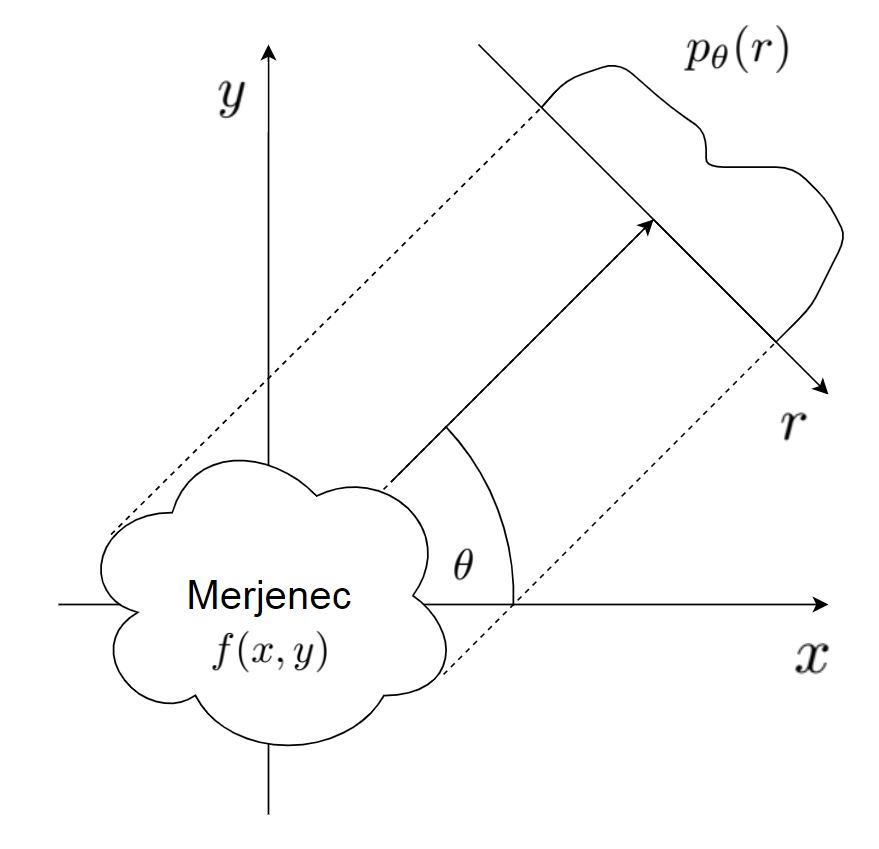
\includegraphics[width=4.5cm]{fig/FBPderi}}
	\caption{Filtrirana povratna projekcija.}
	\label{fig:fbp_deri}
\end{figure}

Zajete projekcije so nato pretvorjene v frekven?no domeno s pomo?jo Fourier-ove transformacije $P_{\theta}(\omega)$ za vsak kot. Tu nato sledi filtriranje projekcij s frekven?nim odzivom $|\omega|$ tako, da dobimo $g_{\theta}(r) = \int  P_{\theta}(\omega)|\omega|e^{i 2\pi\omega r} d\omega$. S filtriranjem se ?elimo znebiti visokih frekvenc v projekcijah in posledi?no pridobiti kvalitetnej?o rekonstrukcijo. Po filtriranju nato sledi ?e rekonstrukcija v $f'(x,y)$ in sicer tako, da filtrirane inverze Fourier-ove transformacije se?tejemo.

\begin{equation}
f'(x,y) = \frac{1}{2\pi} \int_{0}^{\pi} g_{\theta}(r) (x \cos\theta + y \sin \theta)d\theta
\end{equation}

Ali v diskretni obliki, kjer je $\Delta\theta$ korak diskretizacije:
\begin{equation}
f'(x,y) = \frac{1}{2\pi} \sum\limits_{i=0}^{N-1} \Delta\theta_i g_{\theta_i}(x \cos\theta_i + \sin\theta_i)
\end{equation}

Za potrebe naloge je postopek raz?irjen v tretjo dimenzijo. Na spodnji sliki je prikazan diagram poteka uporabljenjega FBP algoritma.

\begin{figure}[H]
	\centerline{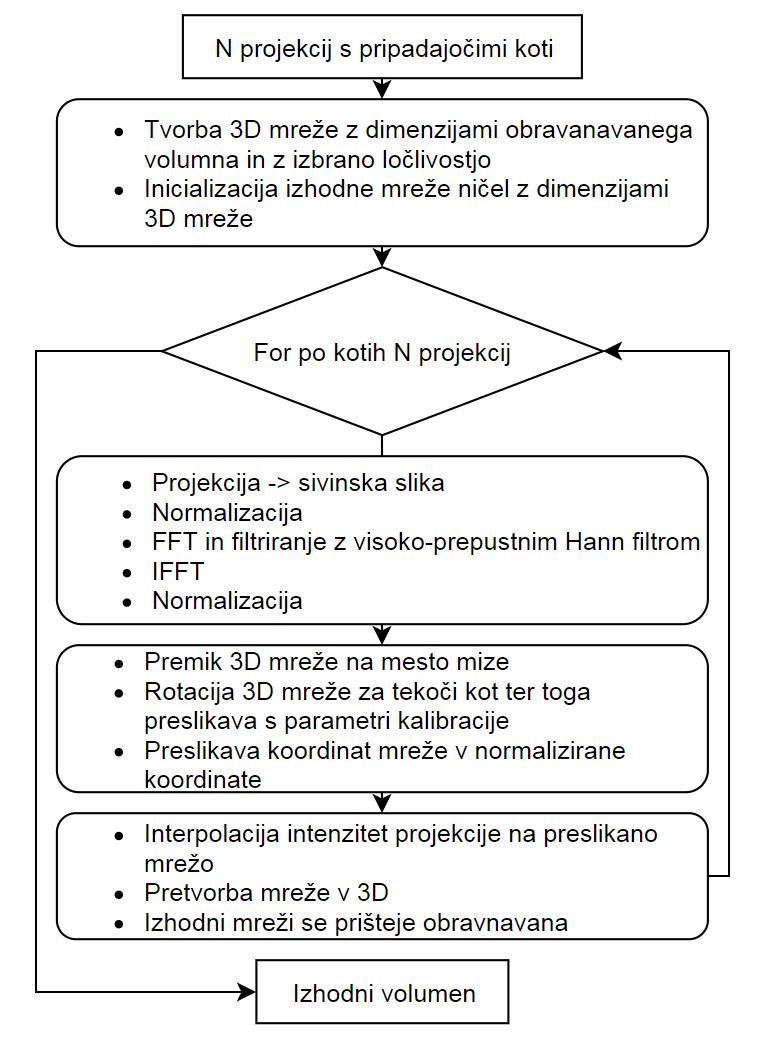
\includegraphics[width=6cm]{fig/FBPflow}}
	\caption{Diagram poteka FBP algoritma.}
	\label{fig:fbp_flow}
\end{figure}

\subsection{Poravnava oblakov to?k}
%
Potek algoritma poravnave to?k je prikazan na sliki ~\ref{fig:alg_poravnava}. Poravnavno izvajamo med dvema oblakoma to?k tako, da enega prilagajamo na drugega. Na za?etku oba oblaka to?k postavimo v koordinatno izhodi??e. Nato izvajamo optimizacijo prileganja na razli?ih rotacijah prilagajo?ega oblaka. Slednje je izvedeno tako, da prilagajo? oblak rotiramo po 20 stopinj in v vsaki legi izvajamo optimizacijo. To ponavljamo za 360 stopinj. Na koncu med vsemi izberemo poravnano lego, ki nam zagotavlja najmanj?o povpre?no napako. 

\begin{figure}[H]
	\centerline{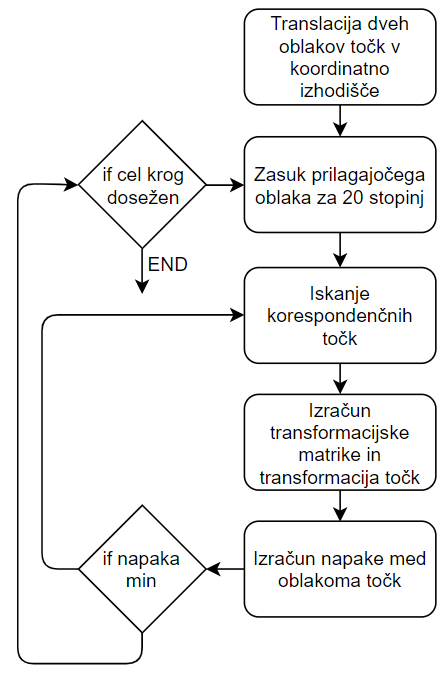
\includegraphics[width=4.5cm]{fig/alg_poravnava}}
	\caption{Potek algoritma poravnave.}
	\label{fig:alg_poravnava}
\end{figure}

\section{Zajem slik}
Sistem s katerim smo izvajali rekonstrukcijo je blokovno prikazan na sliki ~\ref{fig:blokovna}. Objekt, ki ga ?elimo skonstruirati postavimo na vrtljivo pozicionirno mizo. Iz zgornje strani navzdol svetimo s homogeno, difuzno osvetlitvijo. Objekta direktno ne osvetljujemo, saj je namen osvetlitve predvsem osvetlitev ozadja z enakomerno intenziteto. Cilj je dose?i ?imve?jo razliko v intenziteti med opazovanim objektom in zaslonom. Za ta namen je med objekt in svetilko postavljena svetlobna ovira. Slike smo zajemali z Raspberry Pi kamero v osi na objekt in na osvetljeno ozadje. Pred kamero je dodan filter za namen filtriranja okoli?ke svetlobe.

\begin{figure}[H]
	\centerline{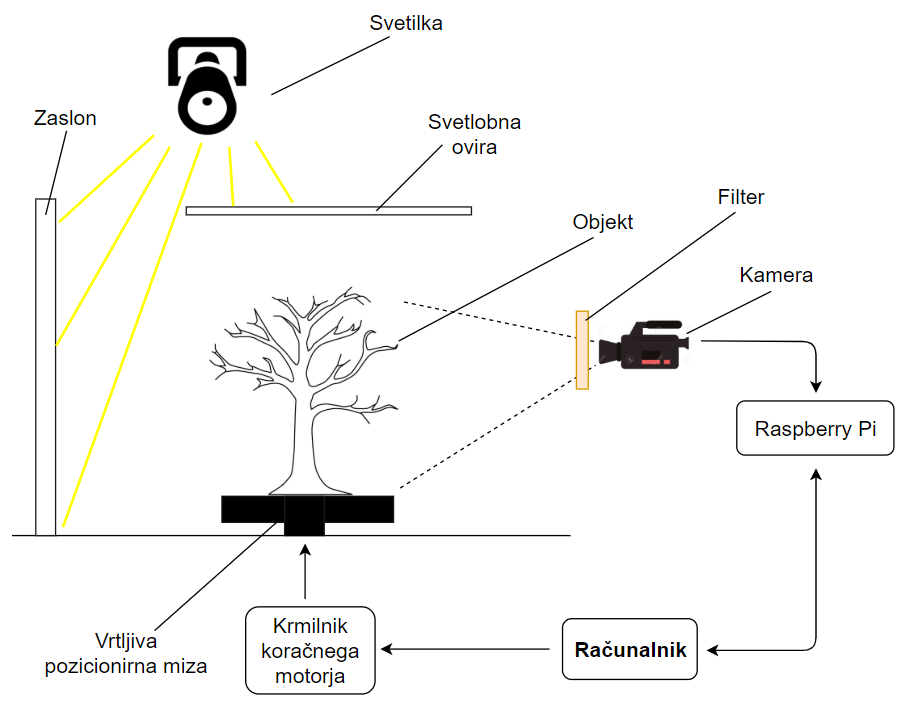
\includegraphics[width=8.2cm]{fig/blokovna_sistem}}
	\caption{Semioperacijska shema sistema.}
	\label{fig:blokovna}
\end{figure}
%
 Celoten proces zajemanja krmilnimo z ra?unalnikom. Ta je ?i?no povezan na krmilnik s katerim upravljamo rotirajo?o pozicionirno mizo. Prav tako je ra?unalnik brez?i?no povezan na Raspberry Pi. Ta zajete slike po?ilja na ra?unalnik. Objekt rekonstruiramo tako, da ga postavimo na predvideno mesto. Nato lahko pri?nemo z zajemom slik. Najprej inicializiramo kamero na za?etne vrednosti. Nastavimo ISO na 200, svetlost na 45 in resolucijo na 900x1000.  Objekt obra?amo po za?rtanih zasukih. Po vsakem izvedenem zasuku posnamemo eno sliko, ki se nato brez?i?no prenese iz Raspberry Pi-ja na ra?unalnik. Postopek ponavljamo dokler objekta ne poslikamo v rangu celotnega kroga. Zajete slike ob znanih kotih zasuka se kasneje uporabijo za 3D rekonstrukcijo. V tabeli ~\ref{tab:komponente} so zapisane vse glavne komponente, ki so zajete v postavljenem sistemu. Manj?e komponente kot so vijaki in nosilci v tabeli niso zajeti.

\begin{center}
	\centering
	\captionsetup{singlelinecheck = false, justification=justified}
	\captionof{table}{Komponente sistema.} 
	\label{tab:komponente} 
\begin{tabular}{|c|c|}
	\hline
	\textbf{Komponenta} & \textbf{Podrobnosti}                            \\ \hline
	Raspberry Pi        & Raspberry Pi 3 Model B                          \\ \hline
	Svetilka            & Halogenska svetilka (12V)            \\ \hline
	Zaslon              & Bela ravna plo??a                               \\ \hline
	Krmilnik            & Fischertechnik stage control                \\ \hline
	Kamera              & RP Cam V2-8 MP,1080p \\ \hline
	Svetlobni filter    & Ozkopasovni filter         \\ \hline
	Svetlobna ovira     & Kartonasta zavesa                \\ \hline
		Pozicionirna miza   & Fischertechnik rotary stage                     \\ \hline
\end{tabular}
\end{center}
Primer zajete slike obravnavanega objekta z opisanim sistemom je prikazan na sliki ~\ref{fig:zajeta_slika}. S slike lahko vidimo dober kontrast objekta in precej?njo razliko v barvi in svetlosti objekta proti ozadju. 

\begin{figure}[H]
	\centerline{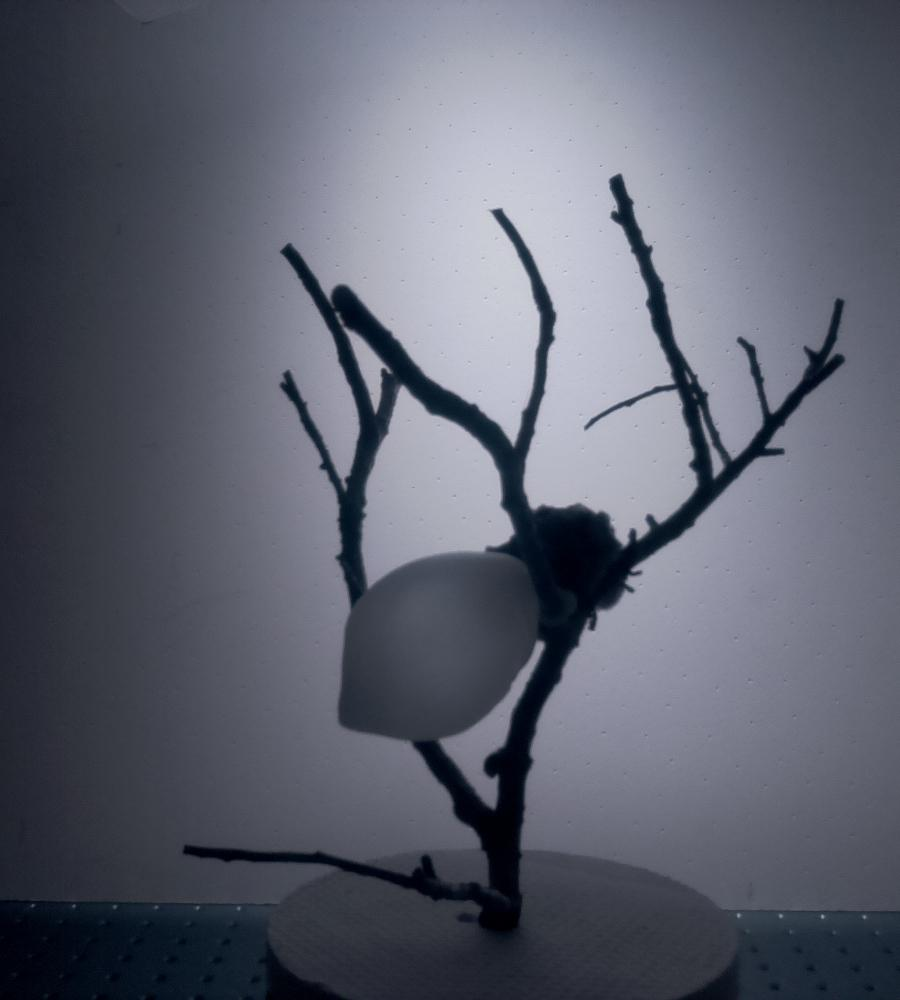
\includegraphics[width=4.2cm]{fig/zajeta_slika}}
	\caption{Zajeta slika.}
	\label{fig:zajeta_slika}
\end{figure}

\section{Rezultati}
\subsection{Vpliv kontrasta}
Testirali smo kako svetlobna pregrada vpliva na rekonstrukcijo oblaka to?k. Za ta namen smo vzeli enostaven objekt s stali??a rekonstrukcije. Ta je prikazan na sliki ~\ref{fig:slusalkEE}. Na levi strani je prikazana slika objekta kjer svetlobne ovire nismo uporabili. Razvidnno je, da se od objekta svetloba reflektivno odbiva v kamero. Kamera to zazna kot svetlo intenziteto. Deli objekta, ki so tako osvetljeni se po svetlosti veliko ne razlikujejo od ozadja, na nekaterih delih pa so celo zaznani, kot svetlej?i. Na desni strani je prikazana slika objekta, kjer svetlobno oviro uporabimo. Objekt je v tem primeru bistveno temnej?i od ozadja.

\begin{figure}[H]
	\centerline{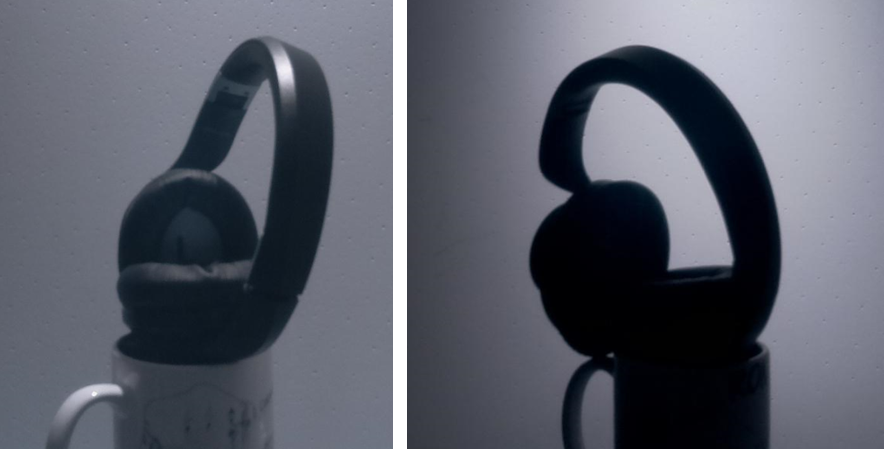
\includegraphics[width=6.2cm]{fig/slusalke_1}}
	\caption{Objekt: a) brez pregrade, b) s pregrado.}
	\label{fig:slusalkEE}
\end{figure}

Na sliki ~\ref{fig:slusalke} sta prikazana rezultata rekonstrukcij brez in z uporabo svetlobne ovire. Opazimo lahko, da je v primeru uporabljene pregrade objekt bistveno lep?e rekonstruiran. V primeru, ko zavese nismo uporabili nam odboji povzro?ajo napa?no reprezentacijo objekta. 



\begin{figure}[H]
	\centerline{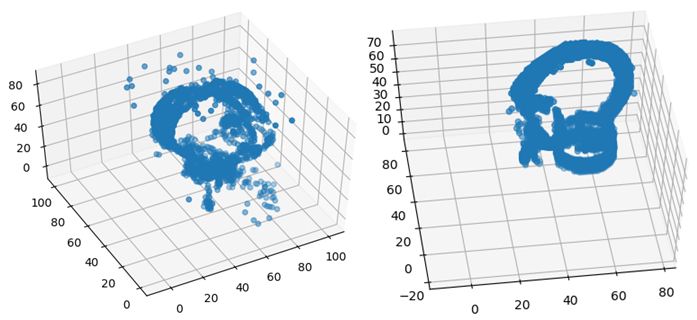
\includegraphics[width=6.2cm]{fig/slusalke}}
	\caption{Rekonstrukcija: a) brez pregrade, b) s pregrado.}
	\label{fig:slusalke}
\end{figure}


\subsection{?tevilo zajetih slik}
Dvakrat smo rekonstruirali isti predmet. Enkrat na podlagi 30 slik in drugi? na podlagi 90 slik. Opazovali smo kako ?tevilo zajetih slik vpliva na rekontrukcijo. Na sliki ~\ref{fig:slika_90_30} je ?isto na levi strani prikazan skeniran objekt, na sredini objekt rekonstruiran na podlagi 90 slik in na desni objekt rekonstruiran na podlagi 30 slik. Vidimo, da je dobimo bolj?o obliko na podlagi ve?ih slik. Za prikaz celotnega objekta v obeh primerih bi bilo potrebno prilagoditi meje upragovanja. 
%
\begin{figure}[H]
	\centerline{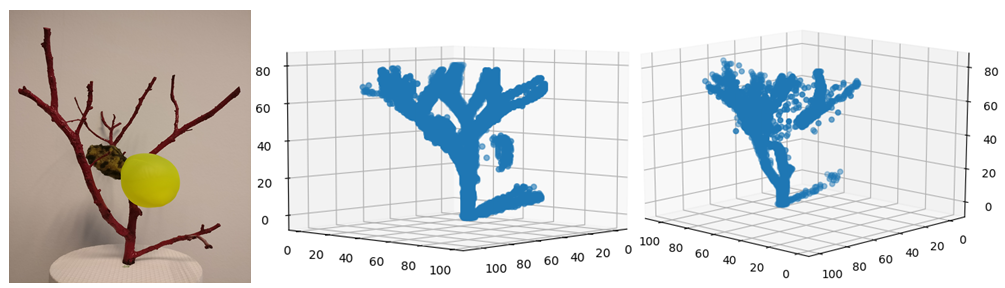
\includegraphics[width=8cm]{fig/slika_90_30}}
	\caption{a) objekt, b) zajetih 90 slik, c) zajetih 30 slik.}
	\label{fig:slika_90_30}
\end{figure}
%
%
\subsection{Poravnava oblakov to?k}
Za dodaten eksperiment smo izvedli medsebojno poravnavo oblakov to?k. Referen?ni oblak to?k smo zajeli z 90 slikami in si zapolnili referen?no lego objekta na pozicionirni mizi. Nato smo izvedli ?e ?est zajemov po 30 slik. Ob vsakem zajemu smo skeniran objekt zasukali za predpisan kot glede na referen?no lego okoli vertikalne osi. Tako smo zajeli oblake to?k zasukane za 45, 90, 135, 180, 225 in 315 stopinj. Na sliki ~\ref{fig:poravnava} sta zaradi preglednosti prikazana le referen?ni oblak in oblak zasukan za 90 stopinj. Na levi strani sta oblaka prikazana pred poravnavo in na desni po poravnavi. 

\begin{figure}[H]
	\centerline{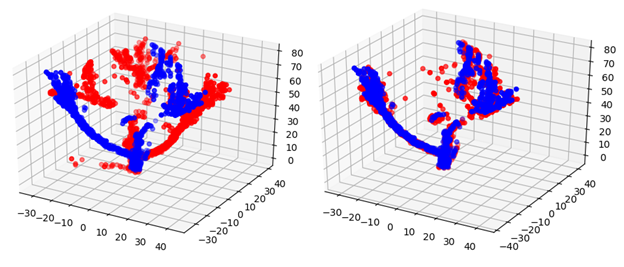
\includegraphics[width=8cm]{fig/poravnava}}
	\caption{a) neporavnana, b) poravnana.}
	\label{fig:poravnava}
\end{figure}
%
Za vse, pod razli?nimi koti zajete oblake to?k, smo izvedli poravnavo. Nato smo iz pridobljene transformacijske matrike izlu??ili rotacijo okoli vertikalne osi. Ker smo poznali kote zasuka objekta glede na referen?no lego, smo jih primerjali s temi pridobljenimi iz transformacijske matrike. Na sliki ~\ref{fig:poravnava_graf} so z rde?o barvo prikazani ro?no dolo?eni zasuki, z modro pa zasuki pridobljeni iz transformacijske matrike. Vidimo, da dobimo z izra?unanimi koti na podlagi transformacijske matrike dokaj zanesljive rezultate. Prileganje testiranih zasukov glede na referen?ne je v rangu petih stopinj. Napaka se verjetno pojavi zaradi napak v pozicionirnem sistemu, nenatan?ne meritve kota glede na referen?no lego in napake v numeri?nem izra?unu.

\begin{figure}[H]
	\centerline{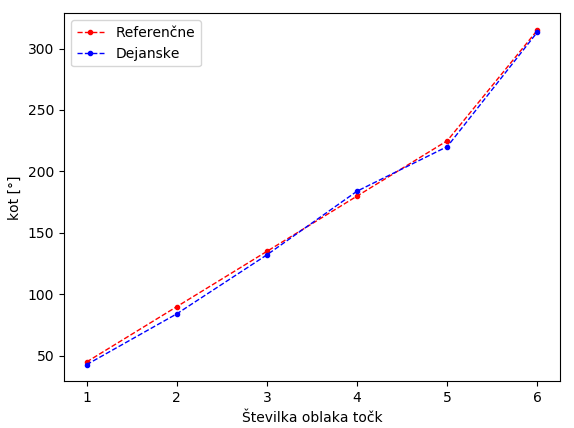
\includegraphics[width=8cm]{fig/graf_poravnave}}
	\caption{Razlika med referen?nimi in dejanskimi koti.}
	\label{fig:poravnava_graf}
\end{figure}

\subsection{Vzvratno in?enirstvo}

Vzvratno in?enirstvo je proces, kjer na podlagi fizi?nega objekta rekonstruiramo njegov model. Model smo dobili tako, da smo z rekonstrukcijo dobljen oblak to?k uvozili v 3D modelirnik Solidworks. Tam smo z uporabo posebnih orodij iz to?k povr?ine predmeta dobili povr?ino sestavljeno iz trikotnikov in posledi?no zaprli vse odprtine tako, da smo dobili zaprto povr?ino. Nato je sledila interpolacija z namenom pridobive gladkej?e povr?ine in transformacija v "trdnino". Po opravljenih korakih smo imeli model v primerni obliki za izvoz v formatu .stl. Omenjeni format se nato uvozi v razslojevalni (angl. \textit{Slicer}), ki napravi G-kodo 3D tiskalnika za tvorbo fizi?nega modela. Na sliki ~\ref{fig:print_slusalke} je na levi strani prikazan natisnjen objekt. Na desni strani je prikazan model pripravljen na tiskanje. Gre za objekt s slike ~\ref{fig:slusalkEE}.

\begin{figure}[H]
	\centerline{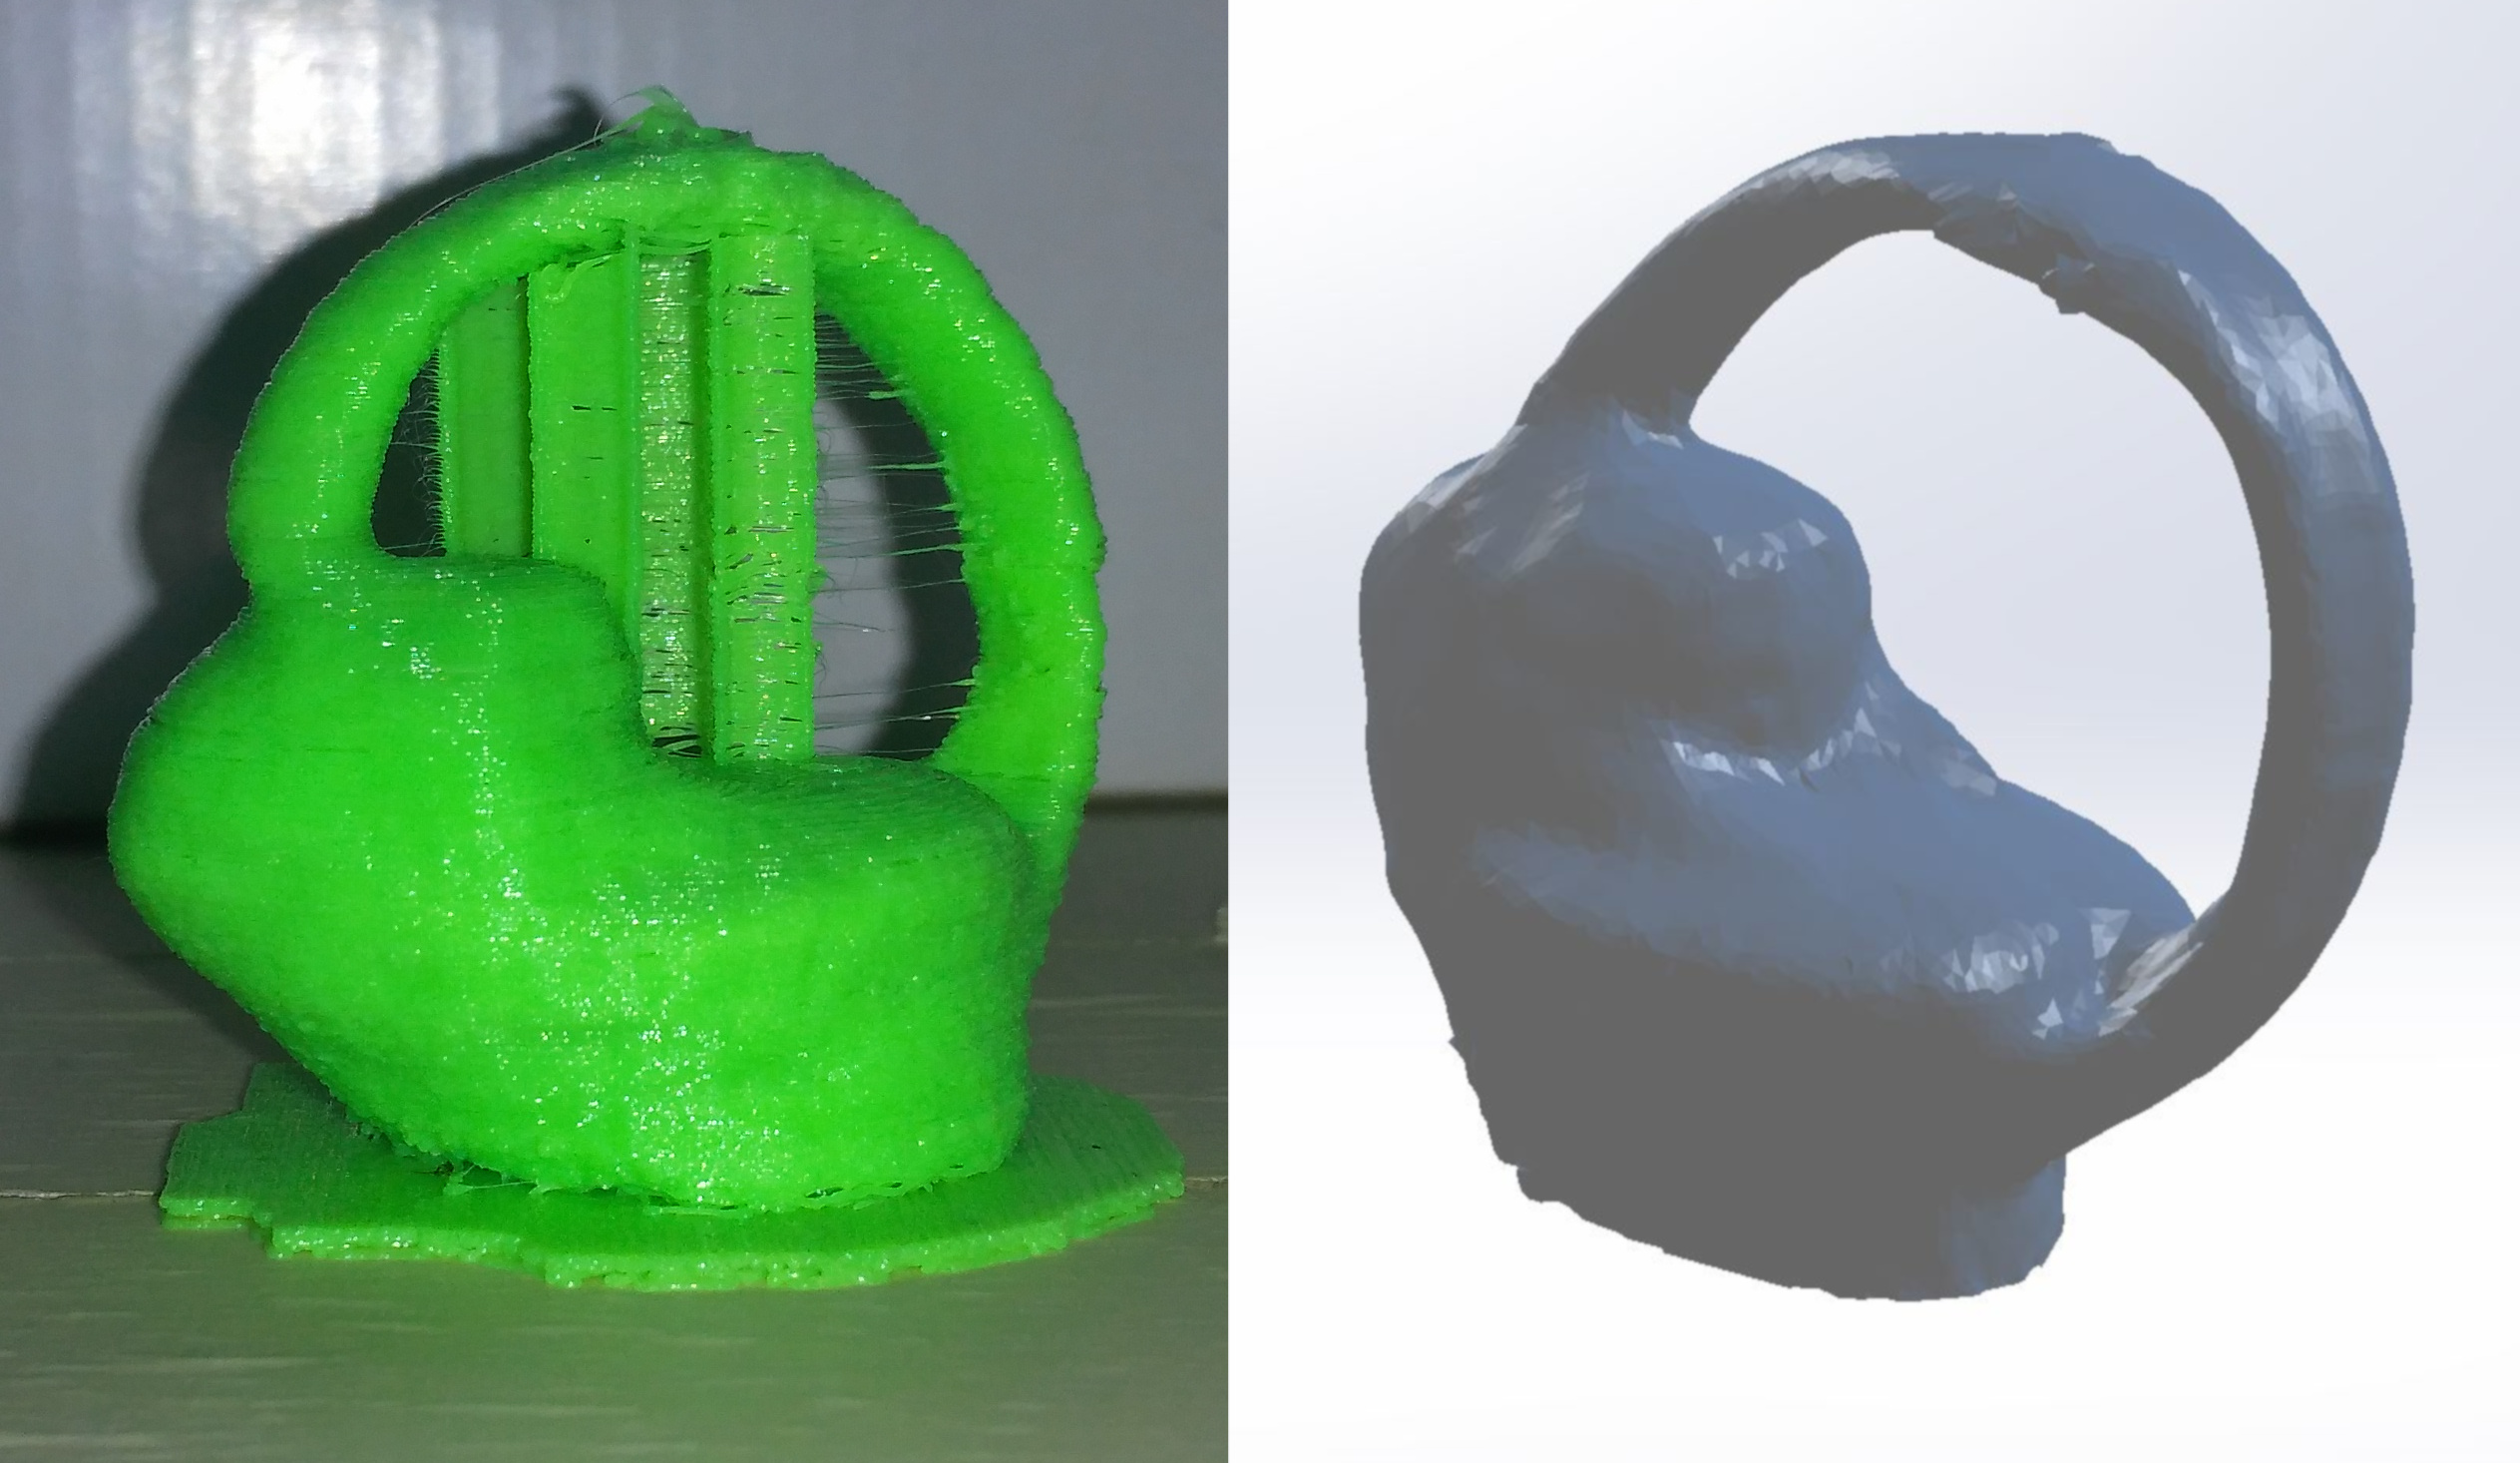
\includegraphics[width=7cm]{fig/print_slusalke}}
	\caption{a) model po tiskanju, b) lupina modela v modelirniku.}
	\label{fig:print_slusalke}
\end{figure}

\section{Zaklju�ki}
Tekom izvajanja naloge smo ugotovili da postopek 3D FBP rekonstrukcije dobro deluje pri popisu predmetov, ki ne vsebujejo majhnih detajlov (slika \ref{fig:slika_90_30}).  Na kvaliteto rekonstrukcije mo?no vplivamo s ?tevilom zajetih slik ter z ustrezno osvetlitvijo, tako se znebimo ?rtastih arftefaktov, ki nastanejo s postopkom FBP. Pri tem pa je potrebno omeniti, da se ?as rekonstrukcije mo?no pove?a z ve?jim ?tevilom slik. S pojmom dobra osvetlitev pa mislimo velik kontrast med ozadejm ter slikanim predmetom. Uporabljen algoritem rekonstrukcije omogo?a tudi grobo dimenzijsko analizo, saj z upo?tevanjem lo?ljivosti dobimo rekonstrukcijo v pribli?nih dimenzijah merjenca.

Poravnava oblakov se je izkazala za izredno uspe?no kot to prikazuje tudi graf na sliki \ref{fig:poravnava_graf}. Pri pretvorbi digitalnega modela v fizi?nega pa smo ugotovili, da na kvaliteto rezultirajo?ega modela mo?no vpliva vrsta algortima za izlu??evanje to?k povr?ine, transformacija oblaka to?k v 3D model ter sam postopek 3D tiskanja.

%Z na?o tehniko rekonstruiranja nismo popisali dovolj dobrih delailov, ?as rekonstrukcije se pove?juje z velikostjo sempljanja, ugotovili smo, da je sistem zelo pomemben + osvetlitev. Pomembno tud ?tevilo slik. Poravnava slik, nam je dobro uspela - lahko ?e ne bi poznali pod kak?nim kotom je poslikal in dobil koliko je zamaknjen glede na referen?no lego.


\begin{thebibliography}{10}
\bibitem{spic1} ?. ?piclin, B. Likar, M. Burmen. {\em Predavanje pri predmetu - Biomedicinske slikovne tehnologije: Rekonstrukcija slik}, \hskip 1em plus 0.5em minus 0.4em \relax Univerza v Ljubljani, 2018.
\bibitem{spic2} ?. ?piclin. {\em Predavanje pri predmetu - Robotski vid: Prileganje modelov na slike}, \hskip 1em plus 0.5em minus 0.4em \relax Univerza v Ljubljani, 2019.
\bibitem{vir1} Moons, Theo, Luc Van Gool.  {\em 3D reconstruction from multiple images part 1: Principles}, \hskip 1em plus 0.5em minus 0.4em \relax Foundations and Trends in Computer Graphics and Vision 4.4: 287-404, 2010.
\bibitem{vir2}Vosselman, George, and Sander Dijkman.   {\em 3D building model reconstruction from point clouds and ground plans}, \hskip 1em plus 0.5em minus 0.4em \relax International archives of photogrammetry remote sensing and spatial information sciences 34.3/W4: 37-44, 2001.
\bibitem{vir3} Woodham, Robert J.  {\em  Photometric method for determining surface orientation from multiple images}, \hskip 1em plus 0.5em minus 0.4em \relax Optical Engineering. 19 (1): 138?141, 1980.
\bibitem{vir4}   {\em Raspberry Pi 3, Model B V1.2 Technical Specifications}, \hskip 1em plus 0.5em minus 0.4em \relax RS Components, 20.9.2017.
\bibitem{vir5}   {\em Fischertechnik Technical Specifications}, \hskip 1em plus 0.5em minus 0.4em \relax fischertechnik GmbH, 2016.
\bibitem{vir6}   {\em https://en.wikipedia.org/wiki/Tomographic\_reconstruction}, \hskip 1em plus 0.5em minus 0.4em \relax Obiskano dne: 24.5.2019 



\end{thebibliography}

		
		
		

\end{document} 